\documentclass[conference]{IEEEtran}

\usepackage{cite}
\usepackage{amsmath,amssymb,amsfonts}
\usepackage{algorithmic}
\usepackage{graphicx}
\usepackage{textcomp}
\usepackage{xcolor}
\usepackage{tikz}
\usetikzlibrary{arrows.meta,positioning,shapes.geometric}

\def\BibTeX{{\rm B\kern-.05em{\sc i\kern-.025em b}\kern-.08em
    T\kern-.1667em\lower.7ex\hbox{E}\kern-.125emX}}

\begin{document}

\title{A Multi-Agent Architecture for Continuous Regulatory Risk Monitoring in the Brazilian Fintech Sector}

% TODO(user): confirm ordering/format of authors and affiliations before submission.
\author{
\IEEEauthorblockN{1\textsuperscript{st} Gabriel Castelo Branco Rocha Alencar Pinto}
\IEEEauthorblockA{
\textit{Dept. of Computer Science} \\
\textit{Universidade Federal de Minas Gerais (UFMG)} \\
Belo Horizonte, Brazil \\
gcastelob.rocha@gmail.com}
\and
\IEEEauthorblockN{2\textsuperscript{nd} Henrique Rotsen Santos Ferreira}
\IEEEauthorblockA{
\textit{Dept. of Computer Science} \\
\textit{Universidade Federal de Minas Gerais (UFMG)} \\
Belo Horizonte, Brazil \\
% TODO(user): replace with Henrique's preferred email/ORCID.
email@example.com}
}

\maketitle

\begin{abstract}
Financial technology companies operating in Brazil must continuously track a high volume of regulatory publications issued by the Banco Central do Brasil (BCB) and the Comissao de Valores Mobiliarios (CVM), a task that is time-consuming and error-prone when performed manually. This paper presents a multi-agent system that automates the collection, analysis, and prioritization of regulatory changes relevant to fintechs and payment institutions. The system is organized as three cooperating agents, Monitor, Analysis, and Alert, orchestrated by a lightweight sequential pipeline. The Analysis Agent extracts structured information, including summaries, effective dates, obligations, and impact estimates, using a large language model (LLM) with a deterministic heuristic fallback that preserves availability when the LLM backend is unreachable. The system persists documents, extractions, and alerts in a relational store, exposes a continuously refreshing dashboard, and is packaged as containerized worker and web services. We evaluate the analysis pipeline on a corpus of 30 real regulatory documents collected from BCB and CVM, comparing a heuristic baseline against two locally hosted LLMs. Results show high agreement on relevance and obligation extraction, but expose a concrete limitation in date extraction that we discuss critically alongside the governance safeguards, namely mandatory human review, source traceability, and confidence scoring, built into the system.
\end{abstract}

\begin{IEEEkeywords}
multi-agent systems, regulatory compliance, large language models, information extraction, financial technology, human-in-the-loop systems
\end{IEEEkeywords}

\section{Introduction}

Brazilian financial regulators publish a steady stream of rules that directly affect how fintechs and payment institutions operate. The Banco Central do Brasil (BCB) issues circulars, resolutions, and normative instructions covering instant payments (Pix), Open Banking and Open Finance, anti-money-laundering and counter-terrorism-financing controls (PLD/FT), fraud prevention, authentication, and prudential regulation, while the Comissao de Valores Mobiliarios (CVM) publishes resolutions, deliberations, and instructions affecting capital markets participants. For a compliance team, missing or misreading one of these publications can mean an unmet deadline, an unimplemented control, or a regulatory sanction. Manually monitoring every publication channel, filtering the ones that matter for a specific business profile, and turning them into actionable obligations does not scale as the volume of regulatory output grows.

At the same time, fully automating this process is undesirable. Large language models can misread a date, omit an obligation, or infer an impact that the source text does not support. A system that silently converts LLM output into binding compliance decisions would trade a slow manual process for a fast but unreliable one. The design problem this paper addresses is therefore not only how to automate regulatory monitoring, but how to do so in a way that remains transparent, traceable to source, and subject to human review before any alert is acted upon.

This paper reports on the design, implementation, and evaluation of a multi-agent system that addresses this problem for the Brazilian fintech sector. The main contributions are:

\begin{itemize}
\item A three-agent pipeline, Monitor, Analysis, and Alert, implemented as a working system rather than a conceptual design, that collects live data from two independent regulatory sources (BCB and CVM).
\item A dual-mode extraction strategy that combines LLM-based information extraction with a deterministic heuristic fallback, so that LLM provider outages degrade output quality gracefully instead of stopping the pipeline.
\item A quantitative evaluation methodology, consisting of an annotated document corpus and a set of extraction-quality metrics, used to compare a heuristic baseline against two open-weight LLMs served through a university inference endpoint.
\item A containerized deployment that turns the pipeline into a continuously running service, decoupling alert generation from alert consumption through a shared persistence layer and an auto-refreshing dashboard.
\item An explicit governance model that requires human review of every alert, consistent with the system's intended use as a decision-support tool rather than an autonomous compliance system.
\end{itemize}

The remainder of this paper is organized as follows. Section II situates the work with respect to multi-agent systems and large language models. Section III formalizes the monitoring problem. Section IV describes the multi-agent architecture. Section V details the implementation, including the LLM integration strategy and the deployment topology. Section VI describes the evaluation methodology, and Section VII reports and discusses the results. Section VIII discusses governance and ethical considerations, and Section IX concludes with limitations and future work.

\section{Related Work}

Multi-agent systems decompose a complex task into cooperating components with narrower responsibilities, communicating through well-defined interfaces \cite{b1}. The architecture presented in this paper follows this principle at a coarse grain: collection, analysis, and alerting are separated into independent agents that communicate only through persisted, structured data, which keeps each agent independently testable.

The Analysis Agent relies on a large language model to convert unstructured regulatory text into structured fields. This capability builds on the transformer architecture \cite{b2} and on the observation that sufficiently large pretrained language models can perform structured extraction and summarization tasks from a natural-language instruction with little or no task-specific training \cite{b3}. Rather than relying on a proprietary hosted model, the system evaluated in this paper uses open-weight models from the Llama family \cite{b4} and the reasoning-oriented DeepSeek-R1 model \cite{b5}, both served locally through Ollama \cite{b6}, which allows the system to run against a self-hosted inference endpoint instead of an external API.

Frameworks such as LangChain and its stateful extension LangGraph \cite{b7} are widely used to orchestrate tool-using and multi-step LLM agents. These frameworks were part of the initial design of this project, as reflected in the dependency manifest, but the final implementation favors a small, hand-written orchestrator over a general-purpose agent framework; Section V-C discusses this design choice in more detail. The web dashboard is built with Streamlit \cite{b8}, and the two data sources monitored by the system are the official BCB \cite{b9} and CVM \cite{b10} websites.

% TODO(user): this section covers the general technical background (multi-agent
% systems, LLMs, and the specific tools used). Add a focused review of prior
% work on regulatory technology (regtech), compliance-monitoring automation,
% and LLM-based extraction applied to legal or regulatory text, citing the
% specific papers you have read for this course, so that no reference is
% listed without having been read in full.

\section{System Overview and Problem Formulation}

The monitoring environment consists of two heterogeneous, continuously updated regulatory sources: the BCB public news API, which returns recent institutional announcements, and the CVM legislation listing, a paginated page of official acts that is collected through HTML scraping. Documents arrive with inconsistent structure and terminology across sources and document types (circulars, resolutions, normative instructions, and public announcements), which motivates a normalization step before any downstream analysis.

The system targets a specific sector profile, fintechs and payment institutions, rather than the full breadth of financial regulation. The profile is defined by a set of keywords (e.g., payment, fintech, card, transfer, payment institution, gateway, wallet, cryptocurrency, open banking, Pix, authentication, security, anti-money-laundering, fraud, compliance, capital, prudential), a set of tracked business activities (payment processing, interbank transfers, digital wallets, crypto-asset custody, consumer credit, Open Banking, authentication and security, regulatory compliance, and regulatory reporting), and a set of risk areas (compliance, security, anti-money-laundering and counter-terrorism-financing, Open Banking, and authentication). This profile is used by the Analysis Agent to judge relevance and estimate impact, and can in principle be replaced to target a different sector.

Formally, the system observes a stream of raw regulatory documents and must produce, for each relevant document, a structured alert containing a priority level, a plain-language summary, the obligations it imposes, the activities and entities it affects, an implementation deadline when one is stated, and a traceable link back to the original source. Success is measured along the dimensions used in Section VI: whether relevant documents are correctly identified, whether dates are extracted correctly, and whether the obligations described in the alert match the obligations present in the source text.

\section{Multi-Agent Architecture}

The system is organized as a linear pipeline of three agents, coordinated by a central orchestrator, with a persistence layer and a dashboard consuming the pipeline's output, as shown in Fig.~\ref{fig:architecture}.

\begin{figure}[t]
\centering
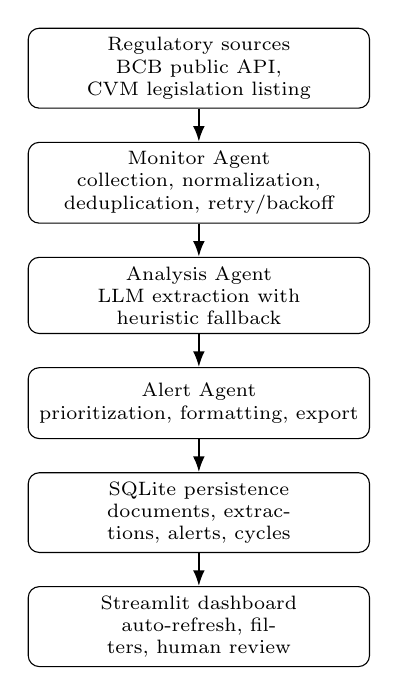
\begin{tikzpicture}[
  node distance=0.42cm,
  box/.style={rectangle, draw, rounded corners, align=center, text width=4.1cm, minimum height=0.9cm, font=\scriptsize},
  arrow/.style={-{Latex[length=2mm]}, thick}
]
\node[box] (sources) {Regulatory sources\\ BCB public API, CVM legislation listing};
\node[box, below=of sources] (monitor) {Monitor Agent\\ collection, normalization, deduplication, retry/backoff};
\node[box, below=of monitor] (analysis) {Analysis Agent\\ LLM extraction with heuristic fallback};
\node[box, below=of analysis] (alert) {Alert Agent\\ prioritization, formatting, export};
\node[box, below=of alert] (db) {SQLite persistence\\ documents, extractions, alerts, cycles};
\node[box, below=of db] (ui) {Streamlit dashboard\\ auto-refresh, filters, human review};

\draw[arrow] (sources) -- (monitor);
\draw[arrow] (monitor) -- (analysis);
\draw[arrow] (analysis) -- (alert);
\draw[arrow] (alert) -- (db);
\draw[arrow] (db) -- (ui);
\end{tikzpicture}
\caption{Overview of the multi-agent monitoring pipeline, from raw regulatory sources to a persisted, human-reviewable alert.}
\label{fig:architecture}
\end{figure}

\subsection{Monitor Agent}

The Monitor Agent is responsible for data acquisition. It collects documents from the BCB public news API, with optional support for a legacy RSS/XML feed, and from the CVM legislation listing, which it paginates up to a configurable page limit. Each item is normalized into a common \texttt{RegulatoryDocument} representation and passed through a content filter that discards items outside the regulatory domain. Deduplication is performed both in memory during a single cycle and against previously persisted documents, matching on URL, document identifier, content hash, and the combination of title, source, and date. Network access to each source is wrapped in a configurable retry-with-backoff policy and a per-source timeout, so that a slow or temporarily unavailable source does not stall the whole cycle.

\subsection{Analysis Agent}

The Analysis Agent receives each collected document and produces an \texttt{ExtractedInfo} record containing a summary, an effective date and an implementation deadline when present, the obligations imposed by the document, the activities and entities it affects, an impact score and description, and a set of recommendations, together with a per-field confidence score and the extraction method used. Extraction can operate in two modes. In \texttt{llm} mode, the agent delegates extraction to a language model through the client described in Section V-B. In \texttt{regex} mode, a deterministic heuristic pipeline performs the same extraction using pattern matching and keyword scoring against the sector profile described in Section III. If the LLM call fails or raises an exception, the agent logs the failure and transparently falls back to the heuristic pipeline, which is the resilience mechanism referenced throughout this paper.

\subsection{Alert Agent}

The Alert Agent consolidates each \texttt{ExtractedInfo} record into a \texttt{StructuredAlert} and assigns a priority level using a deterministic rule that combines the estimated impact score with the urgency of the implementation deadline:

\begin{itemize}
\item \textsc{Critical}: deadline within 7 days, or impact score above 0.9.
\item \textsc{High}: deadline within 30 days, or impact score above 0.7.
\item \textsc{Medium}: deadline within 90 days, or moderate impact score.
\item \textsc{Low}: otherwise.
\end{itemize}

A deliberate design decision excludes deadlines that have already elapsed from automatic escalation to \textsc{Critical}, to avoid flooding reviewers with alerts for obligations that are already overdue and whose urgency framing would otherwise be misleading. The Alert Agent also formats each alert for human triage and exports alerts, individually or as a consolidated per-cycle report, in JSON, CSV, HTML, and PDF.

\subsection{Orchestrator}

The three agents are coordinated by a central orchestrator, \texttt{RegulatoryMonitoringSystem}, which executes a four-stage cycle: document collection and persistence, analysis with content-hash-based caching to avoid re-analyzing unchanged documents, alert generation and persistence, and persistence of a cycle summary. The orchestrator can run a single bounded cycle, useful for testing with a document limit, or run continuously through a \texttt{--watch} mode that repeats the cycle at a configurable interval, catching and logging per-cycle exceptions so that a single failure does not terminate the worker process.

\subsection{Data Model}

All state is persisted in a relational store with four tables: \texttt{documents}, storing collected items and their processing status; \texttt{extractions}, storing structured analysis output keyed by document; \texttt{alerts}, storing prioritized alerts together with their human-review status; and \texttt{monitoring\_cycles}, storing a summarized history of each execution cycle. This persistence layer is what allows the Monitor Agent's deduplication, the Analysis Agent's caching, and the dashboard's history view to operate independently of any single running process.

\section{Implementation}

\subsection{Technology Stack}

The system is implemented in Python. Data collection relies on \texttt{requests} for HTTP access, \texttt{BeautifulSoup} and \texttt{lxml} for HTML parsing of the CVM listing, and \texttt{feedparser} for the optional legacy RSS source. Persistence uses SQLite accessed directly through the standard library, wrapped by a repository class. The dashboard is built with Streamlit. Deployment is containerized with Docker and Docker Compose. Table~\ref{tab:codebase} summarizes the size of the codebase at the time of writing.

\begin{table}[t]
\caption{Codebase size by component}
\label{tab:codebase}
\centering
\begin{tabular}{|l|r|}
\hline
\textbf{Component} & \textbf{Lines of code} \\
\hline
Agents (\texttt{monitor}, \texttt{analysis}, \texttt{alert}) & 1{,}570 \\
\hline
Utilities (LLM client, repository, evaluation) & 1{,}425 \\
\hline
Orchestrator (\texttt{main.py}) & 405 \\
\hline
Dashboard (\texttt{app.py}) & 457 \\
\hline
\textbf{Total production code} & \textbf{3{,}863} \\
\hline
Unit tests (9 modules, 53 test cases) & 869 \\
\hline
\end{tabular}
\end{table}

\subsection{LLM Integration and Resilience}

The \texttt{RegulatoryLLM} client abstracts over two backend protocols: an Ollama-compatible endpoint, accessed through \texttt{/api/chat} with a custom API-key header, and an OpenAI-compatible endpoint, accessed through \texttt{/chat/completions}. Both backends are wrapped with a retry-with-backoff policy, a local per-minute rate limiter, and a response normalizer that maps heterogeneous provider output onto a single, stable JSON schema consumed by the Analysis Agent. Two open-weight models were evaluated against a university-hosted Ollama proxy: \texttt{llama3.2:3b}, chosen for low latency, and \texttt{deepseek-r1:8b}, chosen for stronger reasoning at higher latency. When any part of this path fails, either because the endpoint is unreachable, the request times out, or the response cannot be parsed into the expected schema, the Analysis Agent falls back to the heuristic extraction path described in Section IV-B instead of failing the document.

\subsection{From Agent Framework to Custom Orchestrator}

The project's dependency manifest still lists \texttt{langchain}, \texttt{langgraph}, and \texttt{chromadb}, reflecting the initial design intent to build the pipeline on top of an established agent-orchestration framework with vector-store-backed retrieval. The implementation that was ultimately shipped, however, does not import any of these libraries: the orchestrator is a small, explicit Python pipeline, and the LLM client is a direct HTTP integration rather than a framework-mediated one. Although the specific reasons for this shift are not formally documented in the project history, the resulting design has a clear advantage for a system of this size: every step of the pipeline, from retry logic to fallback behavior, is explicit and can be unit-tested in isolation, which is harder to guarantee when control flow is mediated by a general-purpose agent framework. This trajectory, from framework-based prototyping to a bespoke, narrowly scoped implementation, is a design decision worth surfacing explicitly rather than treating the initial dependency choice as a fixed constraint.

\subsection{Dashboard}

The dashboard, implemented in Streamlit, exposes a metrics overview, a cycle history view, and a filterable alert list. The header, the metrics view, and the alert list are each wrapped in a Streamlit fragment configured to refresh automatically at a configurable interval, so that the dashboard reflects new alerts without a full page reload or manual action from the user. Alerts can be filtered by regulator, priority, affected activity, review status, and minimum confidence. Marking an alert as reviewed is persisted back to the repository, so that the human-review state survives across dashboard sessions. Alerts and consolidated cycle reports can be downloaded directly from the dashboard in the same formats produced by the Alert Agent.

\subsection{Deployment}

The system is packaged as a single multi-stage Docker image: a builder stage installs Python dependencies into a virtual environment, and a slim runtime stage copies only that environment and the application code, running as a non-root user. Docker Compose defines two services built from this image: a \texttt{worker} service running the orchestrator in continuous mode, and a \texttt{web} service running the Streamlit dashboard with a health check against its status endpoint. Both services share a single named volume containing the SQLite database, which is what allows the worker to keep producing alerts independently of whether the dashboard is being viewed, and allows the dashboard to serve up-to-date data without direct access to the worker process. The volume persists across container restarts and is not removed by a normal shutdown of the services.

\section{Evaluation Methodology}

\subsection{Annotated Corpus}

Evaluation uses a corpus of 30 real documents collected from BCB and CVM through the same Monitor Agent used in production, stored as one JSON record per line. Each record contains the document's metadata and content together with a \texttt{gold} block used as ground truth, comprising expected relevance, effective date, implementation deadline, obligations, affected activities, and impact score. The corpus used in this evaluation is flagged internally as \texttt{seeded\_auto\_needs\_human\_review}: the gold labels were generated automatically by the pipeline itself as a starting point and had not yet been manually validated at the time of this evaluation. This is an important qualification for how the results in Section VII should be read.

\subsection{Metrics}

Four groups of metrics are computed against the corpus. Relevance is measured as precision, recall, and F1 against the gold relevance label. Date extraction is measured as accuracy for the effective date, accuracy for the implementation deadline, and their average. Obligation extraction is measured as precision, recall, and F1 based on text similarity between extracted and gold obligations. Deadline estimation is additionally measured as the mean absolute error, in days, between the extracted and gold implementation deadline, when both are available.

\subsection{Experimental Setup}

Three configurations were compared on the same 30-document corpus: a heuristic-only baseline, corresponding to the Analysis Agent's fallback path, and the same pipeline configured to use the \texttt{llama3.2:3b} and \texttt{deepseek-r1:8b} models through the Ollama endpoint. All three configurations were evaluated with the same sample size and the same evaluation script, and telemetry recorded during LLM-backed runs includes counts of successful LLM calls and of silent fallbacks to the heuristic path, so that any comparison can be checked for fallback-induced bias.

\section{Results and Discussion}

Table~\ref{tab:results} summarizes the most recent evaluation run available at the time of writing.

\begin{table}[t]
\caption{Extraction quality across configurations (n = 30 documents)}
\label{tab:results}
\centering
\begin{tabular}{|l|c|c|c|}
\hline
\textbf{Configuration} & \textbf{Relevance F1} & \textbf{Obligations F1} & \textbf{Date acc.} \\
\hline
Heuristic baseline & 1.00 & 1.00 & 0.00 \\
\hline
LLM \texttt{llama3.2:3b} & 1.00 & 1.00 & 0.00 \\
\hline
LLM \texttt{deepseek-r1:8b} & 1.00 & 1.00 & 0.00 \\
\hline
\end{tabular}
\end{table}

Two results stand out and require careful interpretation rather than face-value reporting. First, relevance and obligation F1 scores of 1.00 across all three configurations, including the heuristic baseline, are not evidence that extraction is perfect. Because the gold labels for this corpus were auto-seeded by the same heuristic pipeline being evaluated, the heuristic configuration is effectively being scored against its own output, and the LLM configurations inherit whatever bias that introduces. These numbers should be read as a validation that the evaluation pipeline itself is wired correctly, not as a benchmark of extraction quality, until the gold corpus is manually curated as planned.

Second, date accuracy of 0.00 across all three configurations, including both LLMs, is a genuine and reproducible finding rather than an artifact of the self-seeded gold set: even where the gold date itself was auto-generated, none of the three configurations reproduced it, which points to a systematic mismatch, most likely in date formatting or parsing, between what the agents extract and what the evaluation script expects. This is the clearest concrete limitation surfaced by this evaluation and the highest-priority item for follow-up work, since a date-extraction failure directly undermines the deadline-based prioritization logic described in Section IV-C.

A further threat to validity is LLM endpoint instability: the shared university inference endpoint used for evaluation is not dedicated infrastructure, and transient timeouts observed during development can silently trigger the heuristic fallback described in Section V-B. Because the evaluation script records fallback counts precisely for this reason, any future comparison between the heuristic baseline and an LLM configuration should be reported alongside its fallback rate to rule out the LLM configuration having silently degraded into the heuristic path for part of the run. Finally, with only 30 documents from a single collection window, these results should be treated as a pilot evaluation rather than a statistically robust comparison between models.

\section{Governance and Ethical Considerations}

The system is explicitly designed as a decision-support tool rather than an autonomous compliance system, and this framing is enforced structurally rather than left as a guideline. Every alert requires human review before it is considered actioned, and the dashboard persists this review state rather than treating an alert as resolved once generated. Confidence scores attached to each extracted field are surfaced to the reviewer as an auxiliary signal and are not used to auto-approve or suppress alerts. Every alert retains a traceable link back to its source document, so a reviewer can always verify a claim against the original regulatory text rather than the system's summary of it. The priority rule described in Section IV-C deliberately avoids automatically escalating already-overdue deadlines to \textsc{Critical}, since doing so could create a misleading sense of urgency for an obligation whose original deadline has already passed and whose handling likely requires case-by-case judgment rather than an automated alert. Together, these choices reflect an explicit position that the system does not, and should not, replace legal or compliance counsel, and that language-model output must be treated as a draft to be verified rather than a finding to be trusted.

\section{Conclusion and Future Work}

This paper presented a multi-agent system for regulatory risk monitoring in the Brazilian fintech sector, built around three cooperating agents for collection, analysis, and alerting, a dual LLM-and-heuristic extraction strategy that degrades gracefully under LLM failure, and a containerized deployment that runs the pipeline continuously while serving a live dashboard to human reviewers. An evaluation against a corpus of 30 real BCB and CVM documents showed that the evaluation infrastructure itself is functional, but also surfaced two findings that should shape near-term priorities: the current gold corpus is not yet suitable as a quality benchmark because it was self-seeded rather than independently annotated, and date extraction currently fails across all evaluated configurations, heuristic and LLM alike.

Future work follows directly from these findings. The highest priority is manually curating the annotated corpus into an independent gold set, after which the model comparison should be re-run, ideally in a time window where the shared inference endpoint is stable and fallback events can be minimized. The obligation-extraction metric, currently based on simple text similarity, should be refined to better tolerate paraphrasing. The root cause of the systematic date-extraction failure should be diagnosed directly, since it is likely a narrower bug rather than a fundamental limitation of either extraction strategy. Finally, the export and reporting layouts should be polished ahead of a final presentation, and the sector profile described in Section III could be generalized or parameterized to extend coverage beyond fintechs and payment institutions.

\section*{Acknowledgment}

The authors thank Prof. Antonio Alfredo Ferreira Loureiro and the Department of Computer Science at UFMG for the course context and the shared Ollama inference proxy used during development and evaluation of this system.

\begin{thebibliography}{00}
\bibitem{b1} M. Wooldridge, \emph{An Introduction to MultiAgent Systems}, 2nd ed. Chichester, U.K.: Wiley, 2009.
\bibitem{b2} A. Vaswani, N. Shazeer, N. Parmar, J. Uszkoreit, L. Jones, A. N. Gomez, L. Kaiser, and I. Polosukhin, ``Attention is all you need,'' in \emph{Advances in Neural Information Processing Systems (NeurIPS)}, 2017, pp. 5998--6008.
\bibitem{b3} T. B. Brown \emph{et al.}, ``Language models are few-shot learners,'' in \emph{Advances in Neural Information Processing Systems (NeurIPS)}, 2020.
\bibitem{b4} H. Touvron \emph{et al.}, ``Llama 2: Open foundation and fine-tuned chat models,'' \emph{arXiv:2307.09288}, 2023.
\bibitem{b5} DeepSeek-AI \emph{et al.}, ``DeepSeek-R1: Incentivizing reasoning capability in LLMs via reinforcement learning,'' \emph{arXiv:2501.12948}, 2025.
\bibitem{b6} Ollama, ``Ollama: Get up and running with large language models locally,'' GitHub repository. [Online]. Available: https://github.com/ollama/ollama
\bibitem{b7} LangChain, ``LangChain documentation.'' [Online]. Available: https://python.langchain.com
\bibitem{b8} Streamlit Inc., ``Streamlit documentation.'' [Online]. Available: https://docs.streamlit.io
\bibitem{b9} Banco Central do Brasil. [Online]. Available: https://www.bcb.gov.br
\bibitem{b10} Comissao de Valores Mobiliarios. [Online]. Available: https://www.gov.br/cvm
\end{thebibliography}

\end{document}
